
%----------------------------------------------------------------------------------------
%	PACKAGES AND OTHER DOCUMENT CONFIGURATIONS
%----------------------------------------------------------------------------------------

\documentclass[]{article}
\usepackage{graphicx}
\usepackage{subcaption} 
\usepackage{multirow}
\usepackage{booktabs}
\usepackage{ragged2e}


%----------------------------------------------------------------------------------------
%	PACKAGES AND OTHER DOCUMENT CONFIGURATIONS
%----------------------------------------------------------------------------------------

\usepackage{amsmath,amsfonts,stmaryrd,amssymb} % Math packages

\usepackage{enumerate} % Custom item numbers for enumerations

\usepackage[ruled]{algorithm2e} % Algorithms

\usepackage[framemethod=tikz]{mdframed} % Allows defining custom boxed/framed environments

\usepackage{listings} % File listings, with syntax highlighting
\lstset{
	basicstyle=\ttfamily, % Typeset listings in monospace font
}

%----------------------------------------------------------------------------------------
%	DOCUMENT MARGINS
%----------------------------------------------------------------------------------------

\usepackage{geometry} % Required for adjusting page dimensions and margins

\geometry{
	paper=a4paper, % Paper size, change to letterpaper for US letter size
	top=2.0cm, % Top margin
	bottom=3cm, % Bottom margin
	left=2.5cm, % Left margin
	right=2.5cm, % Right margin
	headheight=14pt, % Header height
	footskip=1.5cm, % Space from the bottom margin to the baseline of the footer
	headsep=1.2cm, % Space from the top margin to the baseline of the header
	%showframe, % Uncomment to show how the type block is set on the page
}

%----------------------------------------------------------------------------------------
%	FONTS
%----------------------------------------------------------------------------------------

\usepackage[utf8]{inputenc} % Required for inputting international characters
\usepackage[T1]{fontenc} % Output font encoding for international characters

\usepackage{XCharter} % Use the XCharter fonts

%----------------------------------------------------------------------------------------
%	COMMAND LINE ENVIRONMENT
%----------------------------------------------------------------------------------------

% Usage:
% \begin{commandline}
%	\begin{verbatim}
%		$ ls
%		
%		Applications	Desktop	...
%	\end{verbatim}
% \end{commandline}

\mdfdefinestyle{commandline}{
	leftmargin=10pt,
	rightmargin=10pt,
	innerleftmargin=15pt,
	middlelinecolor=black!50!white,
	middlelinewidth=2pt,
	frametitlerule=false,
	backgroundcolor=black!5!white,
	frametitle={Command Line},
	frametitlefont={\normalfont\sffamily\color{white}\hspace{-1em}},
	frametitlebackgroundcolor=black!50!white,
	nobreak,
}

% Define a custom environment for command-line snapshots
\newenvironment{commandline}{
	\medskip
	\begin{mdframed}[style=commandline]
}{
	\end{mdframed}
	\medskip
}

%----------------------------------------------------------------------------------------
%	FILE CONTENTS ENVIRONMENT
%----------------------------------------------------------------------------------------

% Usage:
% \begin{file}[optional filename, defaults to "File"]
%	File contents, for example, with a listings environment
% \end{file}

\mdfdefinestyle{file}{
	innertopmargin=1.6\baselineskip,
	innerbottommargin=0.8\baselineskip,
	topline=false, bottomline=false,
	leftline=false, rightline=false,
	leftmargin=2cm,
	rightmargin=2cm,
	singleextra={%
		\draw[fill=black!10!white](P)++(0,-1.2em)rectangle(P-|O);
		\node[anchor=north west]
		at(P-|O){\ttfamily\mdfilename};
		%
		\def\l{3em}
		\draw(O-|P)++(-\l,0)--++(\l,\l)--(P)--(P-|O)--(O)--cycle;
		\draw(O-|P)++(-\l,0)--++(0,\l)--++(\l,0);
	},
	nobreak,
}

% Define a custom environment for file contents
\newenvironment{file}[1][File]{ % Set the default filename to "File"
	\medskip
	\newcommand{\mdfilename}{#1}
	\begin{mdframed}[style=file]
}{
	\end{mdframed}
	\medskip
}

%----------------------------------------------------------------------------------------
%	NUMBERED QUESTIONS ENVIRONMENT
%----------------------------------------------------------------------------------------

% Usage:
% \begin{question}[optional title]
%	Question contents
% \end{question}

\mdfdefinestyle{question}{
	innertopmargin=1.2\baselineskip,
	innerbottommargin=0.8\baselineskip,
	roundcorner=5pt,
	nobreak,
	singleextra={%
		\draw(P-|O)node[xshift=1em,anchor=west,fill=white,draw,rounded corners=5pt]{%
		Question \theQuestion\questionTitle};
	},
}

\newcounter{Question} % Stores the current question number that gets iterated with each new question

% Define a custom environment for numbered questions
\newenvironment{question}[1][\unskip]{
	\bigskip
	\stepcounter{Question}
	\newcommand{\questionTitle}{~#1}
	\begin{mdframed}[style=question]
}{
	\end{mdframed}
	\medskip
}

%----------------------------------------------------------------------------------------
%	WARNING TEXT ENVIRONMENT
%----------------------------------------------------------------------------------------

% Usage:
% \begin{warn}[optional title, defaults to "Warning:"]
%	Contents
% \end{warn}

\mdfdefinestyle{warning}{
	topline=false, bottomline=false,
	leftline=false, rightline=false,
	nobreak,
	singleextra={%
		\draw(P-|O)++(-0.5em,0)node(tmp1){};
		\draw(P-|O)++(0.5em,0)node(tmp2){};
		\fill[black,rotate around={45:(P-|O)}](tmp1)rectangle(tmp2);
		\node at(P-|O){\color{white}\scriptsize\bf !};
		\draw[very thick](P-|O)++(0,-1em)--(O);%--(O-|P);
	}
}

% Define a custom environment for warning text
\newenvironment{warn}[1][Warning:]{ % Set the default warning to "Warning:"
	\medskip
	\begin{mdframed}[style=warning]
		\noindent{\textbf{#1}}
}{
	\end{mdframed}
}

%----------------------------------------------------------------------------------------
%	INFORMATION ENVIRONMENT
%----------------------------------------------------------------------------------------

% Usage:
% \begin{info}[optional title, defaults to "Info:"]
% 	contents
% 	\end{info}

\mdfdefinestyle{info}{%
	topline=false, bottomline=false,
	leftline=false, rightline=false,
	nobreak,
	singleextra={%
		\fill[black](P-|O)circle[radius=0.4em];
		\node at(P-|O){\color{white}\scriptsize\bf i};
		\draw[very thick](P-|O)++(0,-0.8em)--(O);%--(O-|P);
	}
}

% Define a custom environment for information
\newenvironment{info}[1][Info:]{ % Set the default title to "Info:"
	\medskip
	\begin{mdframed}[style=info]
		\noindent{\textbf{#1}}
}{
	\end{mdframed}
}
 % Include the file specifying the document structure and custom commands

%----------------------------------------------------------------------------------------
%	ASSIGNMENT INFORMATION
%----------------------------------------------------------------------------------------

\title{CS622: Advance Computer Architecture \#1 } % Title of the assignment

\author{Aditya Jain (20111004) | Mahi Agrawal (20111029)\\ 

\texttt{adityaj20@iitk.ac.in | maahi20@iitk.ac.in}\\Group Id: 23
% Author name and email address
} 
\date{Indian Institute of Technology, Kanpur--- \today} % University, school and/or department name(s) and a date

%----------------------------------------------------------------------------------------

\begin{document}

\maketitle % Print the title

%----------------------------------------------------------------------------------------
%	PROBLEM 1
%----------------------------------------------------------------------------------------
\\
\section*{Problem 1} % Numbered section
\\
\textbf{Given the trace file of L1 cache misses for six SPEC CPU 2006 applications, calculate the number of L2 and L3 cache misses for different cache hierarchy policies - inclusion, NINE, and exclusion.}
\begin{table}[h]
\textbf{
\caption{Number of L2 Misses}}
\begin{tabular}{llllllll}
\\
\hline
\multicolumn{1}{|c|}{\multirow{2}{*}{\textbf{Trace File}}} &
  \multicolumn{1}{c|}{\multirow{2}{*}{\textbf{Number of References}}} &
  \multicolumn{3}{c|}{\textbf{Number of L2 Misses}} &
  \multicolumn{3}{c|}{\textbf{L2 Misses Rate (PKR)}} \\ \cline{3-8} 
\multicolumn{1}{|c|}{} &
  \multicolumn{1}{c|}{} &
  \multicolumn{1}{c|}{Inclusive} &
  \multicolumn{1}{c|}{NINE} &
  \multicolumn{1}{c|}{Exclusive} &
  \multicolumn{1}{c|}{Inclusive} &
  \multicolumn{1}{c|}{NINE} &
  \multicolumn{1}{c|}{Exclusive} \\ \hline
\multicolumn{1}{|c|}{bzip2} &
  \multicolumn{1}{c|}{1,06,57,627} &
  \multicolumn{1}{c|}{53,98,166} &
  \multicolumn{1}{c|}{53,97,576} &
  \multicolumn{1}{c|}{53,97,576} &
  \multicolumn{1}{c|}{506.51} &
  \multicolumn{1}{c|}{506.45} &
  \multicolumn{1}{c|}{506.45} \\
\multicolumn{1}{|c|}{gcc} &
  \multicolumn{1}{c|}{1,46,10,811} &
  \multicolumn{1}{c|}{30,36,461} &
  \multicolumn{1}{c|}{30,29,809} &
  \multicolumn{1}{c|}{30,29,809} &
  \multicolumn{1}{c|}{207.82} &
  \multicolumn{1}{c|}{207.37} &
  \multicolumn{1}{c|}{207.37} \\
\multicolumn{1}{|c|}{gromacs} &
  \multicolumn{1}{c|}{34,31,511} &
  \multicolumn{1}{c|}{3,36,851} &
  \multicolumn{1}{c|}{3,36,724} &
  \multicolumn{1}{c|}{3,36,724} &
  \multicolumn{1}{c|}{98.16} &
  \multicolumn{1}{c|}{98.13} &
  \multicolumn{1}{c|}{98.13} \\
\multicolumn{1}{|c|}{h264ref} &
  \multicolumn{1}{c|}{23,48,573} &
  \multicolumn{1}{c|}{9,69,678} &
  \multicolumn{1}{c|}{9,65,624} &
  \multicolumn{1}{c|}{9,65,624} &
  \multicolumn{1}{c|}{412.88} &
  \multicolumn{1}{c|}{411.15} &
  \multicolumn{1}{c|}{411.15} \\
\multicolumn{1}{|c|}{hmmer} &
  \multicolumn{1}{c|}{35,09,765} &
  \multicolumn{1}{c|}{17,43,421} &
  \multicolumn{1}{c|}{17,35,322} &
  \multicolumn{1}{c|}{17,35,322} &
  \multicolumn{1}{c|}{496.73} &
  \multicolumn{1}{c|}{494.43} &
  \multicolumn{1}{c|}{494.43} \\
\multicolumn{1}{|c|}{sphinx3} &
  \multicolumn{1}{c|}{1,07,53,447} &
  \multicolumn{1}{c|}{88,20,349} &
  \multicolumn{1}{c|}{88,15,130} &
  \multicolumn{1}{c|}{88,15,130} &
  \multicolumn{1}{c|}{820.23} &
  \multicolumn{1}{c|}{819.75} &
  \multicolumn{1}{c|}{819.75} 


   \\ \hline
\end{tabular}
\begin{tabbing}
\textit{PKR - Number of L2 misses per 1K references}
\end{tabbing}

\end{table}
\\
\textbf{Observation 1.1: For all six applications, inclusion cache policy has the highest number of both L2 and L3 cache misses.} 
\\\\
Inclusion cache policy performance is worse as it suffers from: 
\begin{itemize}
\item \textbf{Inclusion Victims:} When a line is evicted from the L3 cache, inclusion policy enforces the eviction of that block from L2 cache also. When access hits in the L2 cache, the LRU order of the block is updated only in the target L2 cache set, and the LRU order of the block remains unchanged in the L3 cache. As a result, a block that is receiving a lot of hits in the L2 cache may become LRU in its L3 cache set and may get evicted. So this frequently hit block on the next reference will be miss in both the caches and would be brought from memory. 
\item \textbf{Small effective cache capacity:} In inclusion policy, L3 cache contains all the blocks of L2 cache. This duplication of blocks results in the decrease in the effective cache capacity. In our experiment, the ratio of the size of L2 cache to the L3 cache is 1:4. So effectively only 75\% of L3 cache capacity is available for storing blocks that are not present in the L2 cache.
\end{itemize}
\\
\textbf{NINE and exclusion policy suffered less L2 misses as they are immune to inclusion victims}\\
\smallskip
\textbf{\\Observation 1.2 : The number of L2 Misses in the case of NINE and Exclusion policy are same, where as the number of misses for L3 cache are not same in NINE and exclusion policy.} 
\begin{itemize}
    \item The L2 misses are same in both as an eviction of block in L3 cache does not invalidates the block in L2 cache, where as the L3 misses are different because the effective capacity of L3 cache in case of exclusive policy is greater than the effective capacity in case of NINE policy.
\end{itemize}
\pagebreak
\begin{table}[ht]
\\

\begin{tabular}{|c|c|c|c|c|c|c|c|}

\hline
\multirow{2}{*}{\textbf{Trace File}} & \multirow{2}{*}{\textbf{\begin{tabular}[c]{@{}c@{}}Total \\ References\end{tabular}}} & \multicolumn{3}{c|}{\textbf{Number of L3 Misses}} & \multicolumn{3}{c|}{\textbf{L3 Miss Rate (PKR)}} \\ \cline{3-8} 
                                     &                                                                                       & Inclusive       & NINE           & Exclusive      & Inclusive       & NINE         & Exclusive       \\ \hline
bzip2                                & 1,06,57,627                                                                           & 14,46,388       & 14,45,846      & 8,89,221       & 135.71          & 135.66       & 83.44           \\
gcc                                  & 1,46,10,811                                                                           & 13,73,402       & 13,66,248      & 12,42,825      & 94.00           & 93.51        & 85.06           \\
gromacs                              & 34,31,511                                                                             & 1,70,531        & 1,70,459       & 1,59,306       & 49.70           & 49.67        & 46.42           \\
h264ref                              & 23,48,573                                                                             & 3,42,146        & 3,33,583       & 1,43,686       & 145.68          & 142.04       & 61.18           \\
hmmer                                & 35,09,765                                                                             & 3,91,226        & 3,76,344       & 3,00,047       & 111.47          & 107.23       & 85.49           \\
sphinx3                              & 1,07,53,447                                                                           & 82,07,362       & 82,05,144      & 72,20,777      & 763.23          & 763.02       & 671.48  
\\
\hline       
\end{tabular}
\begin{tabbing}
\textit{PKR - Number of L2 misses per 1K references}
\end{tabbing}
\textbf{
\caption{Number of L3 Misses}}
\end{table}
\\
\textbf{Observation 1.3: 
In the case of L3 caches, we observed the number of misses is least in the exclusive and most in the inclusive cache.} 
\begin{center}
    \textbf{Exclusive L3 misses < NINE L3 misses < Inclusive L3 misses}\\ 
\end{center}
\\
\textbf{Miss rate of the NINE L3 cache is marginally lower than that of inclusive L3 cache.} Since NINE cache also suffers from some decrease in effective cache capacity, this marginal difference is due to the absence of inclusion victims. 
\\
\begin{figure}[!h] 
    \centering
	\begin{subfigure}[b]{7cm} 
		\centering 
		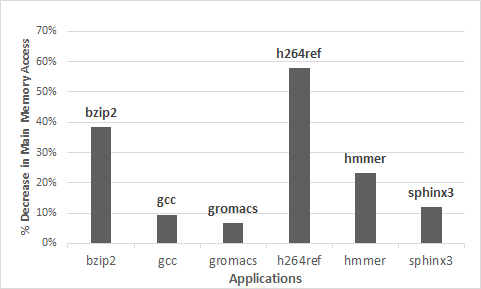
\includegraphics[scale=0.8]{Decrease-memory-access.png}
		\caption{\% decrease in M.M. access in exclusion policy} 
	\end{subfigure} 
	\hspace{0cm} 
	\begin{subfigure}[b]{8cm} 
		\centering 
		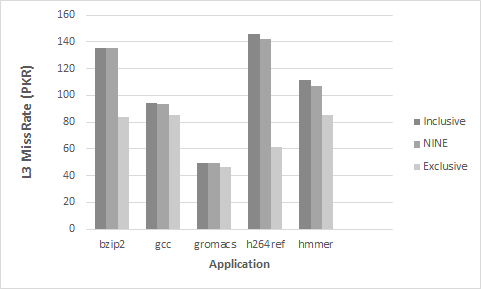
\includegraphics[scale=0.8]{L3_MissRate.png}
		\caption{L3 misses for different cache policies} 
	\end{subfigure}
	
	\caption{}
\end{figure}\\
Figure (1.a) shows the percentage decrease in the number of main memory access for blocks on changing the hierarchy policy from inclusion to exclusion. It shows significant fall for all applications experimented.
\\\\
\textbf{Observation 1.4: The number of misses in the exclusive L3 cache is significantly lower than that of both inclusive and NINE caches.}
\\
\\
Exclusive cache has the largest cache capacity as it does not allows duplication of blocks among the levels of the cache hierarchy. In our experiment: 
\begin{itemize}
    \item Effective exclusive policy capacity = 2560 KB
    \item Effective inclusive policy capacity = 2048 KB
\end{itemize}
\\
Exclusion policy effective cache capacity is \textbf{1.25 times} of the inclusion policy cache capacity. Due to this increase in cache capacity and no inclusion victims in exclusion cache policy enjoys significantly low L3 cache misses.\\
%------------------------------------------------
\pagebreak

\section*{Problem 2}
\textbf{Observation 2.1 : LRU performance is far worse than the Belady's Min policy}

\textbf{\\Explanation}
\begin{itemize}
 \item \textbf{Lru policy} performs worse than the \textbf{Belady's Min policy} as the LRU looks into the past references and \textbf{assumes that the block which is least recently used is unlikely to be requested in near future},so the block which is least recently used is thrown out of the cache,but this \textbf{assumption does not hold always}, due to which it might replace a block which is going to be used in near future,incurring more number of misses. where as \textbf{Belady's Min policy} is an optimal policy,it \textbf{looks into the future references and replaces the block in the cache which is not going to be used for the longest time in future} and hence decreasing the number of misses.
 \item Considering the above points we can say that the assumptions made by LRU were not correct for the large number of evictions from L3 cache, this is also depicted by the table and the graph which shows the total number of misses in the case of belady's Min policy and LRU policy.
 \item This also explains the huge difference between the number of misses and the performance gap between the LRU and belady's  Min policy.
\end{itemize}
\begin{table}[h]
\begin{tabular}{|l|l|l|l|l|}
\hline
\multicolumn{1}{|c|}{\multirow{2}{*}{Trace   File}} &
  \multicolumn{1}{c|}{\multirow{2}{*}{Number of References}} &
  \multicolumn{3}{c|}{Number of L3 Misses} \\ \cline{3-5} 
\multicolumn{1}{|c|}{} &
  \multicolumn{1}{c|}{} &
  Set   Associative LRU &
  Fully Associative LRU &
  Fully Associative Belady \\ \hline
bzip2   & 1,06,57,627 & 14,46,388 & 13,61,401 & 5,36,836  \\
gcc     & 1,46,10,811 & 13,73,402 & 13,69,924 & 9,39,289  \\
gromacs & 34,31,511   & 1,70,531  & 1,69,368  & 1,43,254  \\
h264ref & 23,48,573   & 3,42,146  & 3,35,880  & 1,11,605  \\
hmmer   & 35,09,765   & 3,91,226  & 3,77,024  & 1,53,447  \\
sphinx3 & 1,07,53,447 & 82,07,362 & 83,87,248 & 30,68,580 \\
\hline
\end{tabular}
\caption{Number of L3 Misses}
\end{table}
\begin{table}[h]
\begin{tabular}{|l|l|l|l|l|}
\hline
\multicolumn{1}{|c|}{\multirow{2}{*}{Trace   File}} &
  \multicolumn{1}{c|}{\multirow{2}{*}{Number of References}} &
  \multicolumn{3}{c|}{L3 Miss Rate (PKR)} \\ \cline{3-5} 
\multicolumn{1}{|c|}{} &
  \multicolumn{1}{c|}{} &
  \multicolumn{1}{c|}{Set   Associative LRU} &
  \multicolumn{1}{c|}{Fully Associative LRU} &
  \multicolumn{1}{c|}{Fully Associative Belady} \\ \hline
bzip2   & 1,06,57,627 & 135.714 & 127.74  & 50.371  \\
gcc     & 1,46,10,811 & 93.999  & 93.761  & 64.287  \\
gromacs & 34,31,511   & 49.696  & 49.357  & 41.747  \\
h264ref & 23,48,573   & 145.682 & 143.014 & 47.52   \\
hmmer   & 35,09,765   & 111.468 & 107.421 & 43.72   \\
sphinx3 & 1,07,53,447 & 763.231 & 779.959 & 285.358 \\
\hline
\end{tabular}
\caption{Number of L3 Misses per Thousand Access (PKR)}
\end{table}
\begin{figure}[!h] 
    \centering
		\centering 
	\begin{subfigure}[b]{7cm}	
		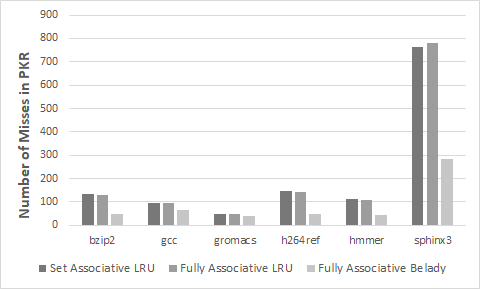
\includegraphics[scale=0.4]{L3missratepkr.png}
		\caption{ Number of L3 Misses per thousand Access} 
\end{subfigure}
\hspace{0cm} 
	\begin{subfigure}[b]{8cm} 
		\centering 
		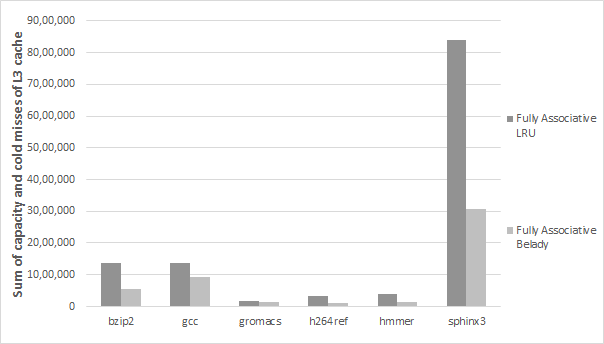
\includegraphics[scale=0.33]{sumofcoldandcapacitymisses.png}
		\caption{L3 misses for different cache policies} 
	\end{subfigure}
\caption{}
\end{figure}\\

\pagebreak
\textbf{\\Observation 2.2 : Belady's Min policy cannot be implemented in real.}
\textbf{\\Explanation}
\begin{itemize}
    \item  \textbf{Belady's Min policy} requires the references to future block request therefore it is \textbf{not possible to implement it in real}, it is significant only for the purpose that one should not scratch his head to find a policy which will give better performance than Belady's Min policy. 
  \end{itemize}
 \textbf{\\Observation 2.3 : Fully associative cache does not always perform better than the set associative cache}
 \textbf{\\Explanation:}
 There are two possible reasons for set associative cache performing much better than the fully associative cache, for the same cache size and block size.
 \begin{itemize}
     \item One reason is that, there might be a possibility that the working set of the blocks accessed is in a such manner that the working set exceeds the size of the cache,in such case there will always be a miss in fully associative cache on each access, where as if the working set is such that although it exceeds the size of the cache, but they are mapped in different sets in a manner, that some sets are not completely occupied by the working set, in this case set associative cache will incur less number of misses than the fully associative cache.
     \item For example consider there is a cache with 4 lines, and one implementation is set associative cache with 2 sets,and 2 ways per set,the other implementation is of fully associative with 4 lines, consider the block accesses as 1,2,4,6,8,1,2,4,6,8... in this fully associative will have 100\% miss rate, where as in set associative there will be a hit on 1, after the initial cold miss. 
    \smallskip
     \item The other reason can be that the block replaced in fully associative cache and set associative cache need not be same. The replaced block in fully associative cache is LRU to the whole cache, where as the replaced block in set associative cache may or may not be LRU to the whole cache, the block is LRU to a specific set. If these two blocks are not same then there is the possibility that the block evicted by the fully associative cache may be accessed in near future, and if it is accessed in near future, then it will incur a miss, where as it will be a hit for set associative cache.
     \smallskip
     \item These two points explains why set associative can have better performance than fully associative cache, and \textbf{this is also shown by the trace file sphinx3}(Table 5)
     
 \end{itemize}
 
\begin{table}[ht]
\centering
\begin{tabular}{|c|c|c|c|c|c|}
\hline
\multirow{2}{*}{Trace   File} & \multicolumn{5}{c|}{Number of L3 Misses}                                         \\ \cline{2-6} 
                              & Set   Associative LRU & Fully Associative LRU & Cold     & Conflict  & Capacity  \\ \hline
bzip2                         & 14,46,388             & 13,61,401             & 1,19,753 & 84,987    & 12,41,648 \\
gcc                           & 13,73,402             & 13,69,924             & 7,73,053 & 3,478     & 5,96,871  \\
gromacs                       & 1,70,531              & 1,69,368              & 7,73,053 & 1,163     & 61,406    \\
h264ref                       & 3,42,146              & 3,35,880              & 63,703   & 6,266     & 2,72,177  \\
hmmer                         & 3,91,226              & 3,77,024              & 75,884   & 14,202    & 3,01,140  \\
sphinx3                       & 82,07,362             & 83,87,248             & 1,22,069 & -1,79,886 & 82,65,179 \\
\hline
\end{tabular}
\caption{L3 Misses Classification, Considering FA LRU}
\end{table}




\begin{table}[h]
\begin{tabular}{|l|l|l|l|l|l|}
\hline
\multicolumn{1}{|c|}{\multirow{2}{*}{Trace   File}} & \multicolumn{5}{c|}{Number of L3 Misses}               \\ \cline{2-6} 
\multicolumn{1}{|c|}{} &
  \multicolumn{1}{c|}{Set   Associative LRU} &
  \multicolumn{1}{c|}{Fully Associative Belady} &
  \multicolumn{1}{c|}{Cold} &
  \multicolumn{1}{c|}{Conflict} &
  \multicolumn{1}{c|}{Capacity} \\ \hline
bzip2                                               & 1446388 & 5,36,836  & 119753   & 9,09,522  & 4,17,083  \\
gcc                                                 & 1373402 & 9,39,289  & 7,73,053 & 4,34,113  & 1,66,236  \\
gromacs                                             & 170531  & 1,43,254  & 7,73,053 & 27,277    & 35,292    \\
h264ref                                             & 342146  & 1,11,605  & 63,703   & 2,30,541  & 47,902    \\
hmmer                                               & 391226  & 1,53,447  & 75,884   & 2,37,779  & 77,563    \\
sphinx3                                             & 8207362 & 30,68,580 & 1,22,069 & 51,38,782 & 29,46,511\\
\hline
\end{tabular}
\caption{L3 Misses Classification,Considering FA Belady}
\end{table}



%----------------------------------------------------------------------------------------

\end{document}
